\begin{figure*}
      \centering
      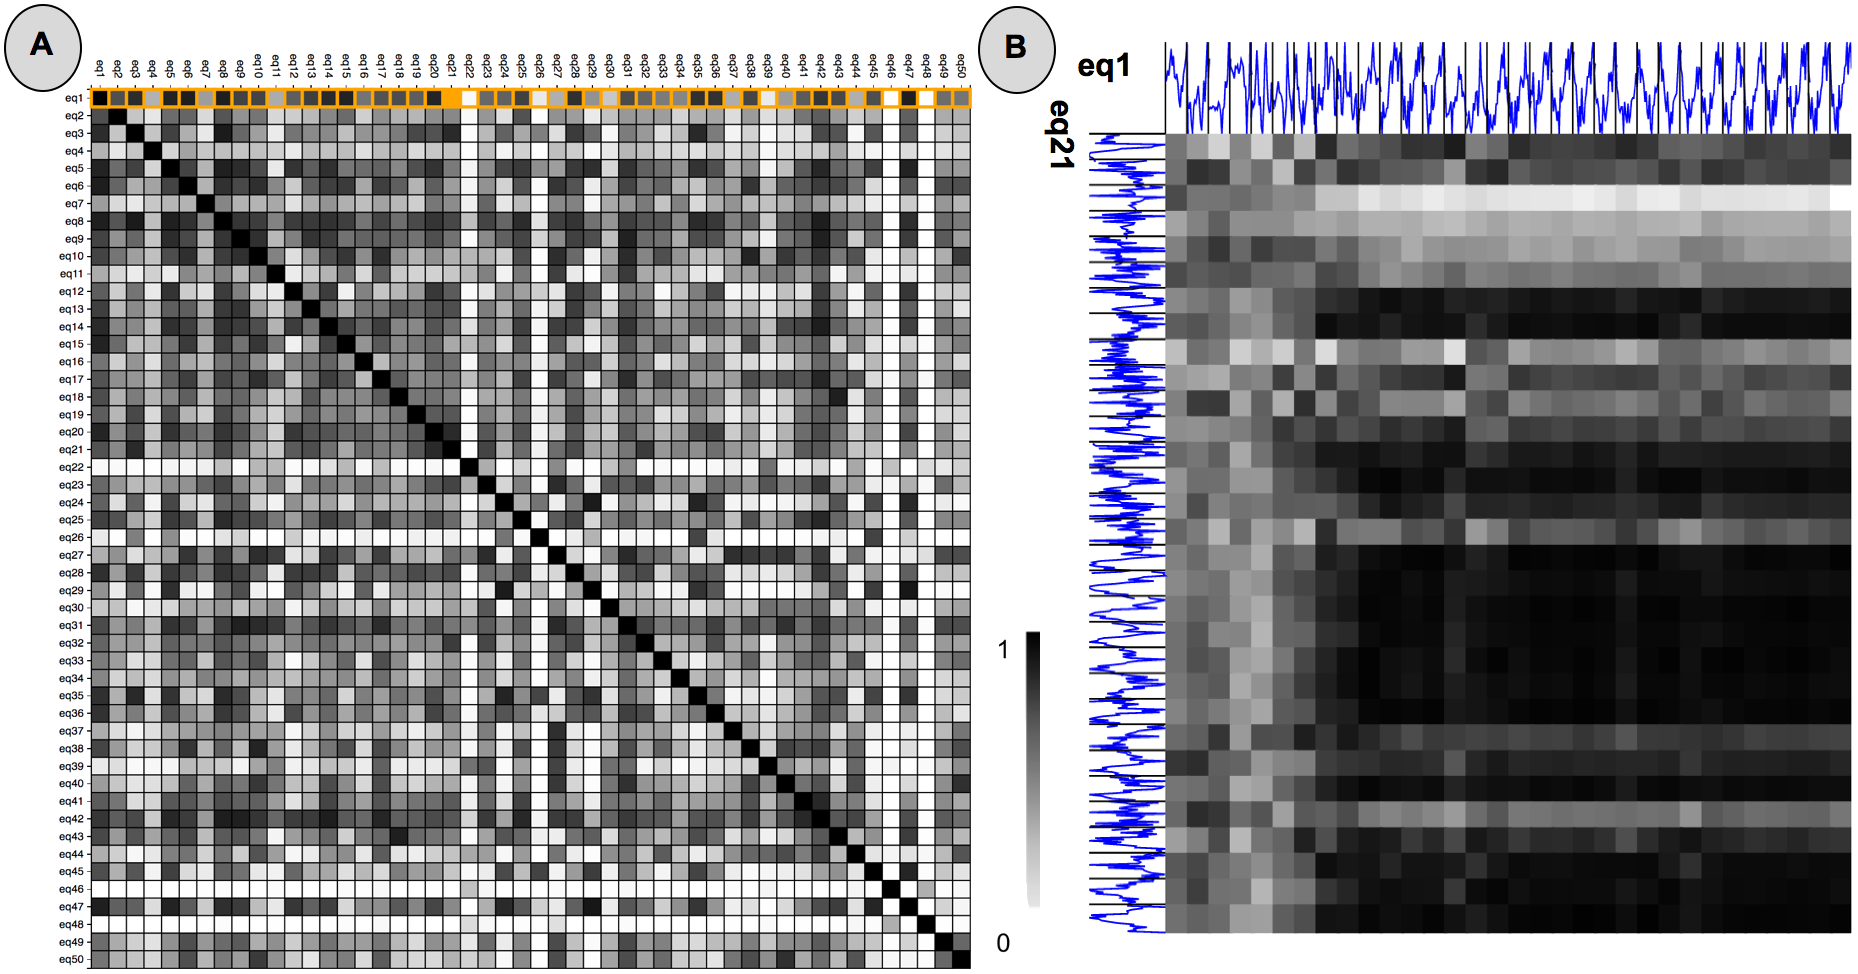
\includegraphics[width=.49\textwidth]{figs/vis1} % first figure itself
      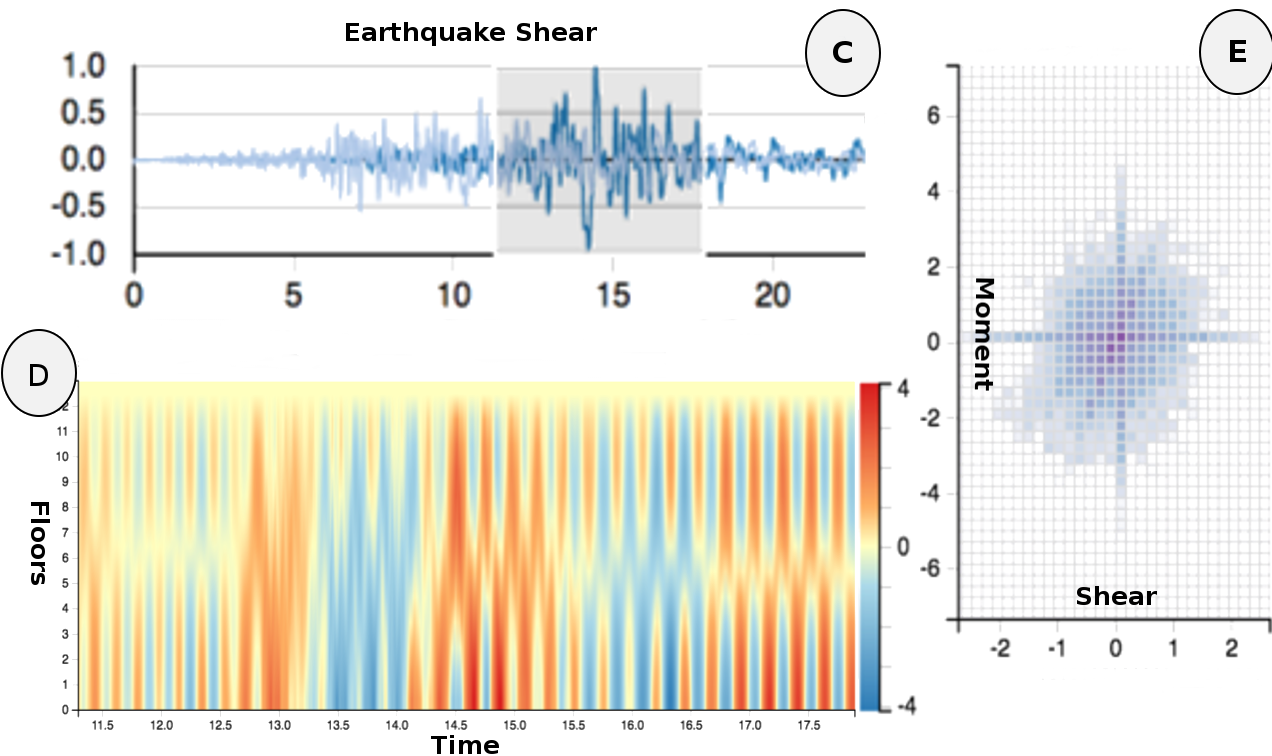
\includegraphics[width=0.37\textwidth]{figs/vis2}
        \caption{Some of the multiple views supporting comparative visualization of earthquake simulations. The response of a building for the entirety of the simulation can be compared to one another, and some earthquakes have more similar responses to others. This gives a comparative overview of all simulations in (A), where a matrix diagram view shows the overall similarities of floor shear across 50 earthquake simulations. In addition, building responses tend to be vibrational and periodic in nature, so segments of an earthquake simulation are compared to one another in (B), where a matrix diagram view demonstrates the similarities between different segments of two earthquake simulations (eq1 and eq21 in view (A)). Analysts can select a portion of the ground acceleration (C) and drill down into a specific earthquake simulation (D), to visualize the response of a single physical variable plotted over time (x coordinate) and building floor (y coordinate). Finally, a 2D histogram can be used to compare two different attributes over the same period of time: how does shear (x coordinate) compare to moment (y coordinate)?\label{fig:teaser}}
\end{figure*}

Through computational simulation, civil engineers can understand how buildings respond to external forces much more efficiently than previously possible.
The simplicity with whcih different scenarios can be simulated and analyzed is attractive, but it is ultimately the source of a new problem: the understanding of the phenomenon is now dependent on the ability to quickly make sense of large amounts of data.

In this poster, we will report on an ongoing collaboration with civil engineers who run a large number of simulations of building responses, and how data analysis and information visualization can highlight interesting patterns in the data.
This problem is especially challenging because of the variety of scales involved. There are multiple earthquakes to be compared to each other; each building's response to an earthquake naturally varies across simulation time, and has different values along different points of the building. There are also periodic phenomena in each simulation, occurring at potentially different periods. Finally, there are multiple physical variables of interest, including shear, moment, and diaphragm forces.

Some of the visualization techniques we using include matrix diagrams and multivariate time series visualizations, as can be seen in Figure~\ref{fig:teaser}. We combine those techniques with classical techniques from signal processing for segmentation, and recent techniques in machine learning for determining similarities between segments of each earthquake simulation.

% Introduction and/or Motivation
%% Analyzing the mechanical structure of different building stories, finding the failing reason when an earthquake attacks a building and investigating the impact of different physical attributes produced by various earthquakes has been a feature of human survival dating back to 230 BC, when ancient Chinese recorded the first earthquake in Puzhou. In efforts to build safer building, understanding earthquake simulation data, for example, the shear stress of each story along the entire time stamps which an earthquake generates when it is shaking a building, is a long-time pursuing for civil engineers. 

%% Nevertheless, currently such tasks can't not be handled and completed perfectly because of the high complexity of the simulation data and the fact that previous work mainly focus on the earthquake itself instead of the simulation data. From visualization perspective, how to visualize such multivariate, multi-scale temporal data remains unclear and potential. In this work, using D3 library~\cite{Bostock:2011:DDD:2068462.2068631},we are trying to design a bunch of visualization views which could help me observe and explore the intricate dataset from different perspectives. Furthermore, we also tried to apply NLP model and kernel methods to these data cubes for comparing them from earthquake level which will be a huge help for the future classification and other machine learning tasks.

%% Besides, the ais of this research is that we also want to compare these earthquake simulation data from different levels. For example, comparing different attributes, what the relation between Shear and Diaphragm Force (two different forces changed during earthquake ) when the earthquake happens. And also what's the behaviour of shear stress among different stories.

% Maybe you want to use a list:

%The rest of the paper isSection~\ref{sec:vis}
